\section{Results}
\label{sec:results}
\begin{figure*}[h!]
     \centering
     % \textbf{\rotatebox{90}{CNN$\,\;$}}
     \begin{subfigure}[b]{0.24\textwidth}
         \centering
         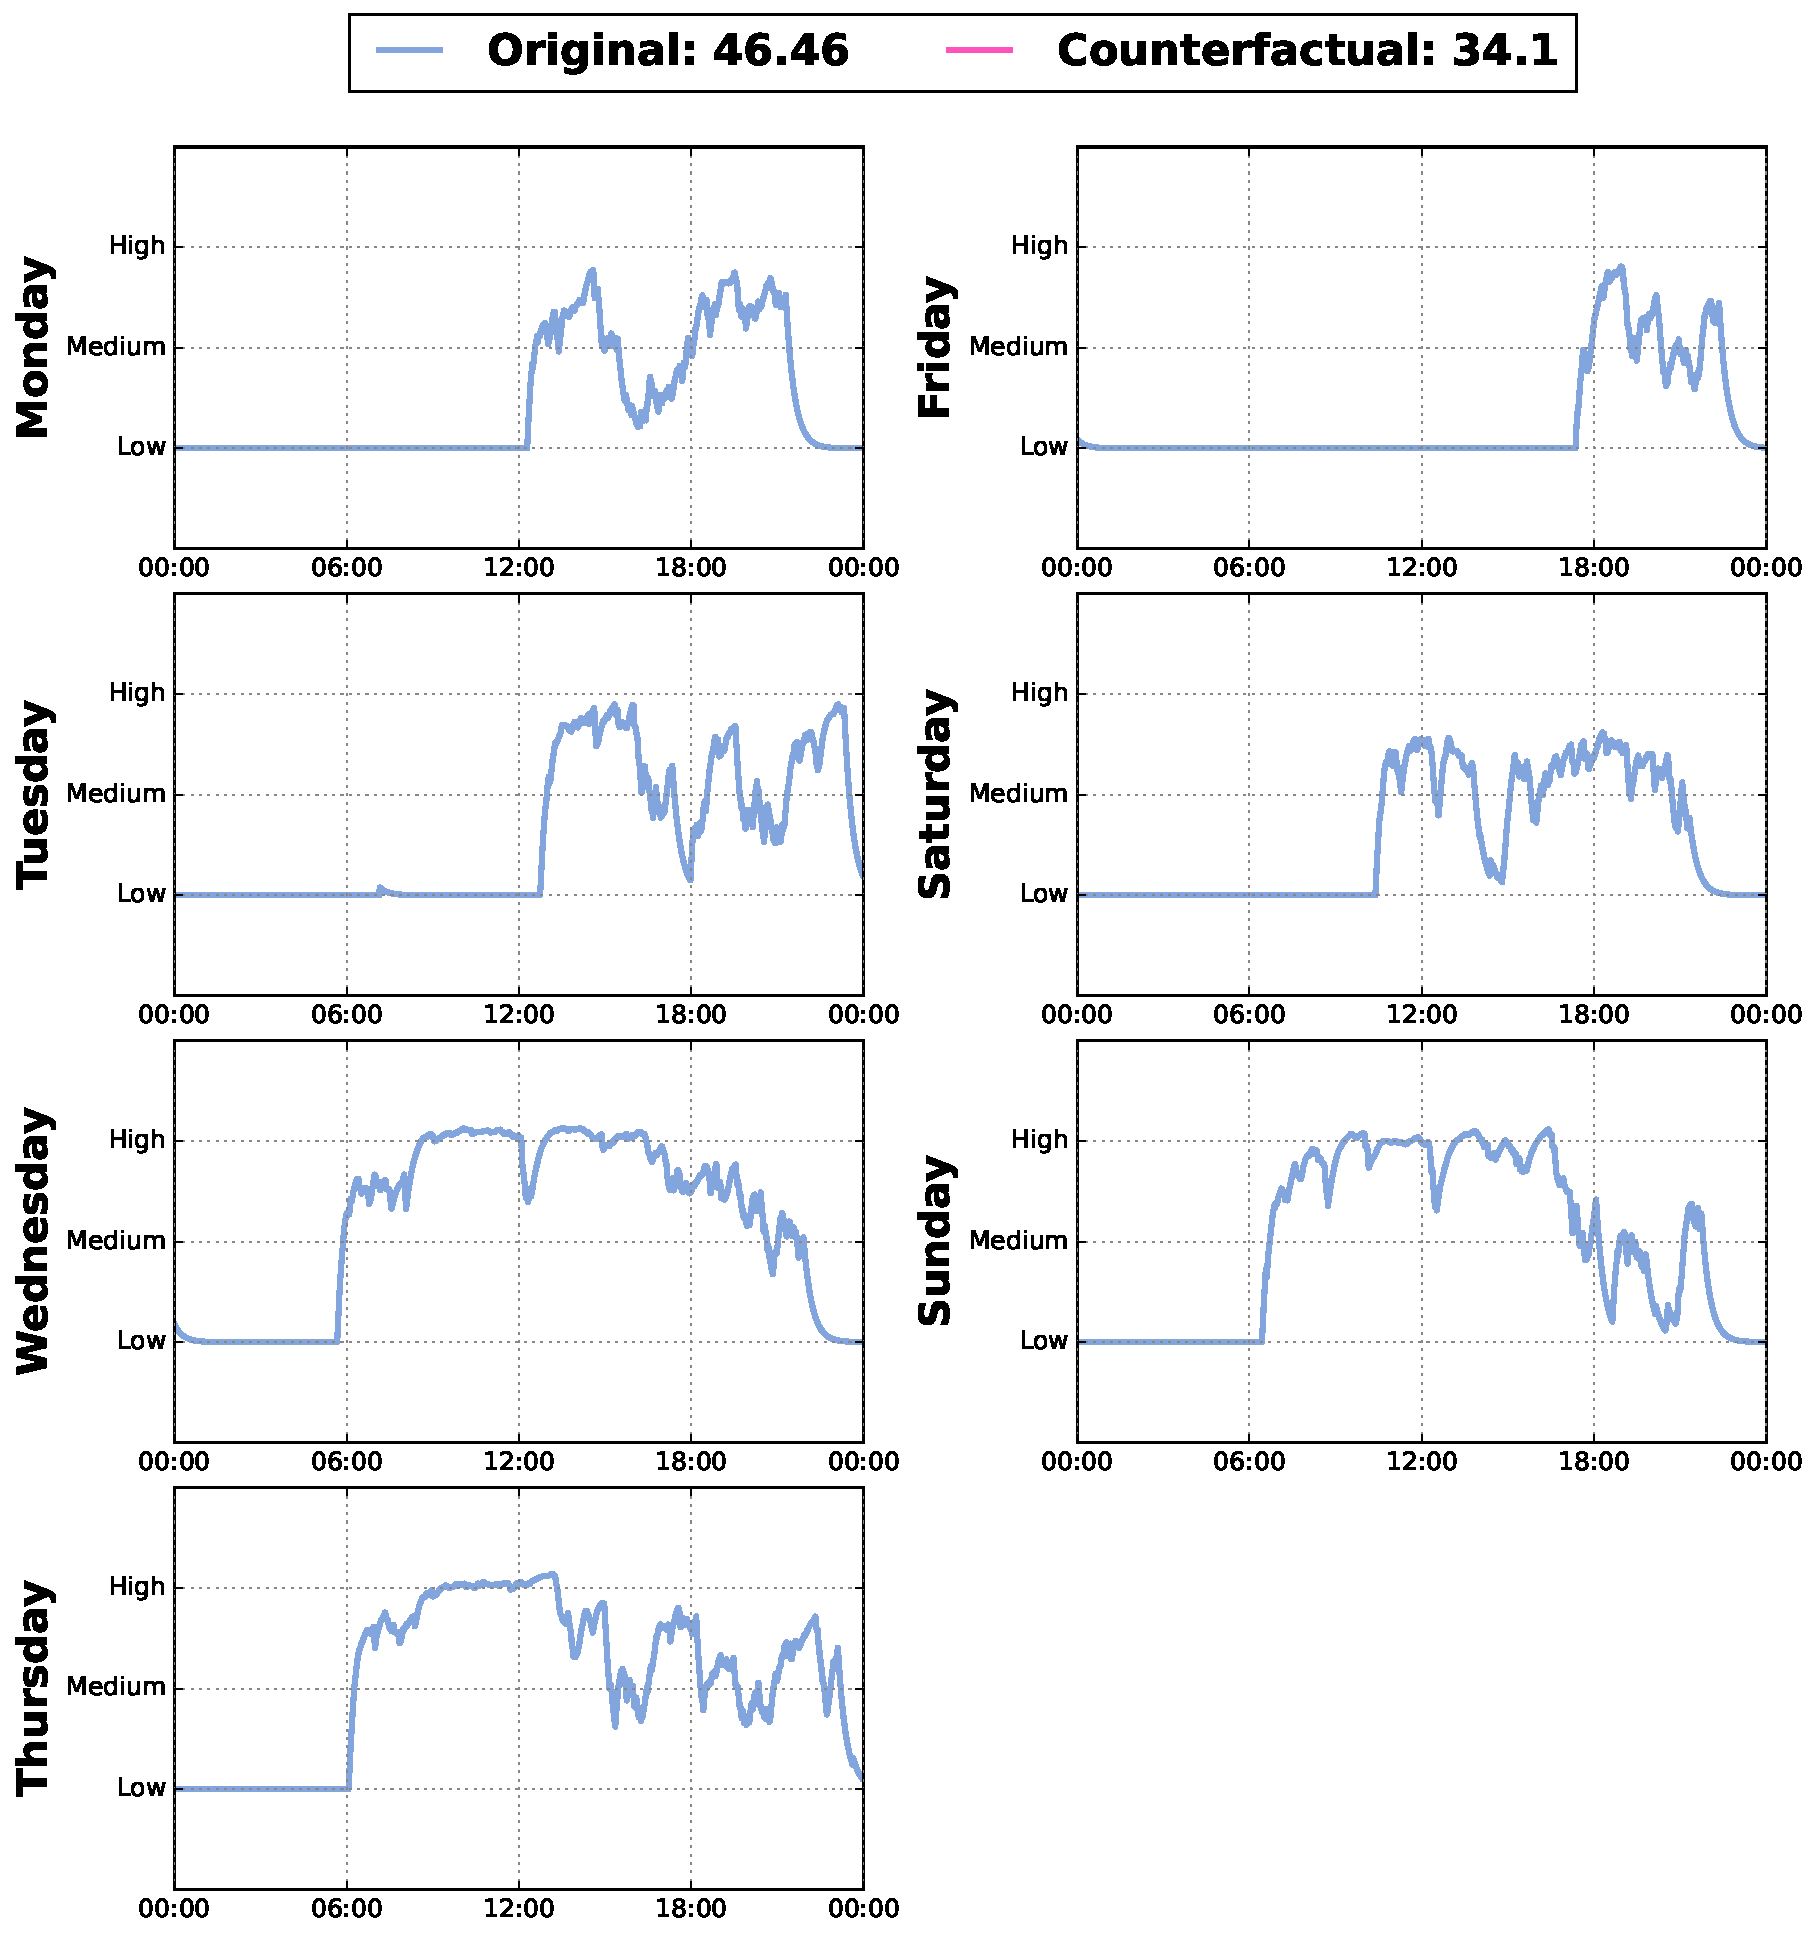
\includegraphics[width=\textwidth]{images/6306/0_6306_TCN_Wachter_cf.pdf}
         \caption{\gls{wachter} Counterfactual}
         \label{fig:cf:wachter}
     \end{subfigure}
     \hfill
     \begin{subfigure}[b]{0.24\textwidth}
         \centering
         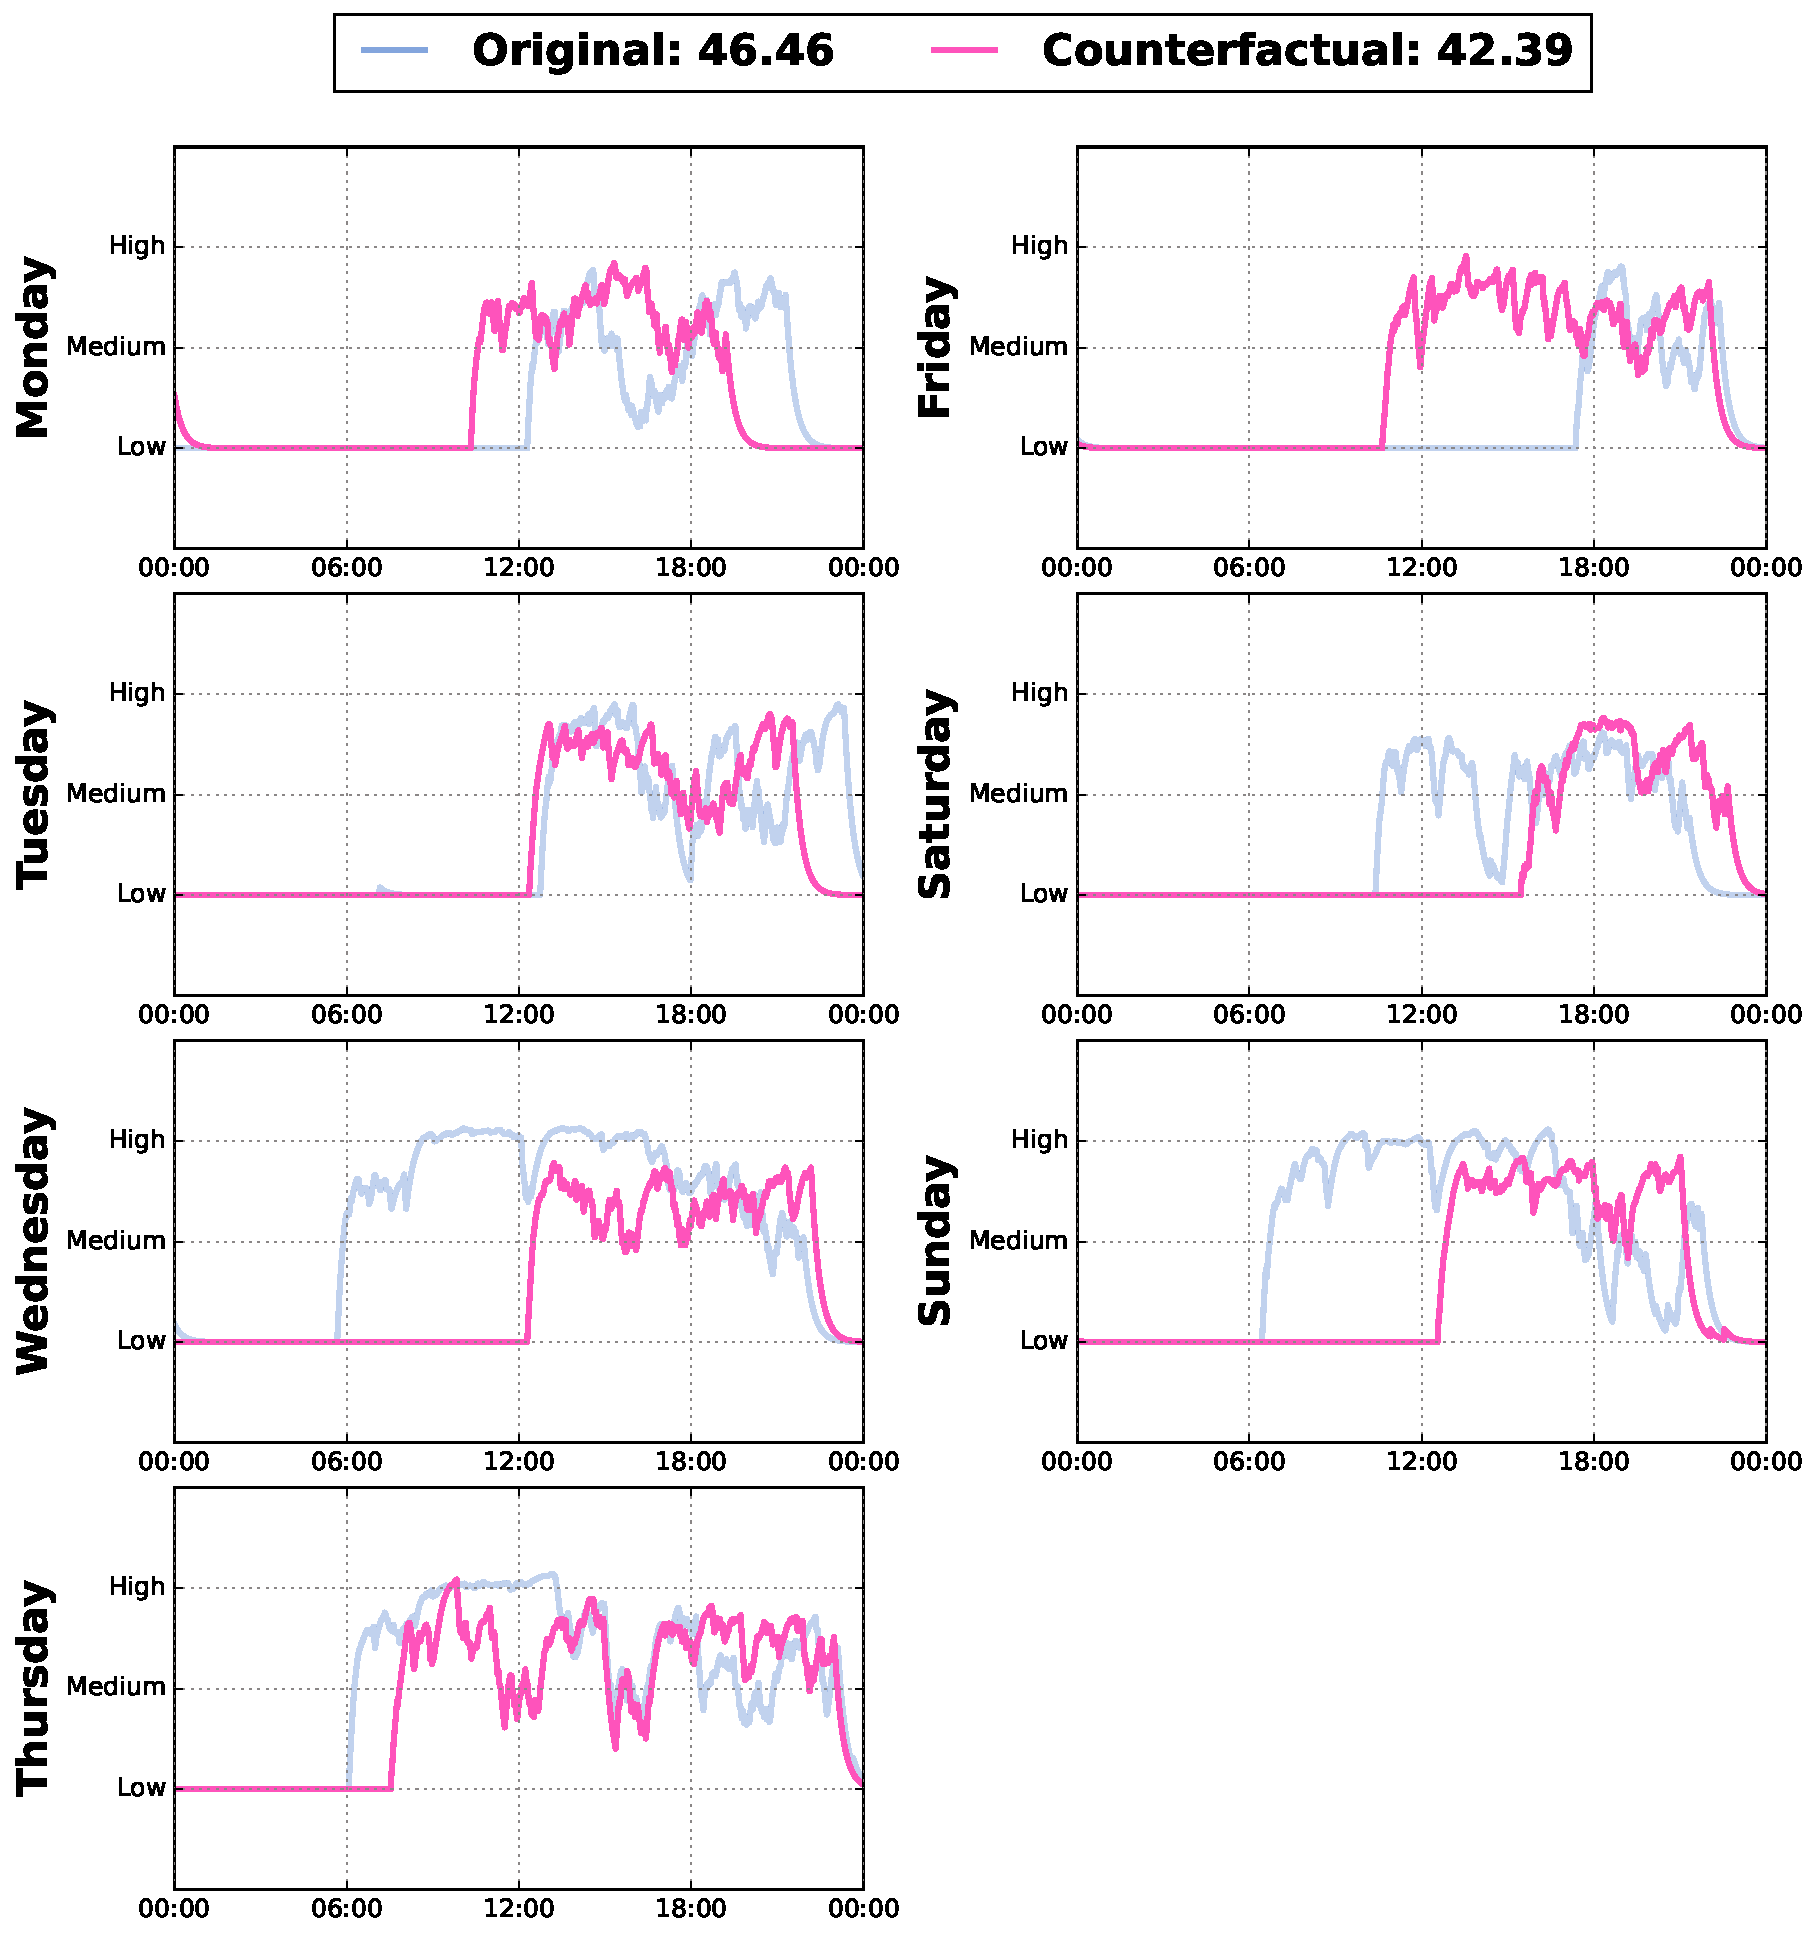
\includegraphics[width=\textwidth]{images/6306/4_6306_TCN_NUN_cf.pdf}
         \caption{NUNR Counterfactual}
         \label{fig:cf:nun}
     \end{subfigure}
     \hfill
     \begin{subfigure}[b]{0.24\textwidth}
         \centering
         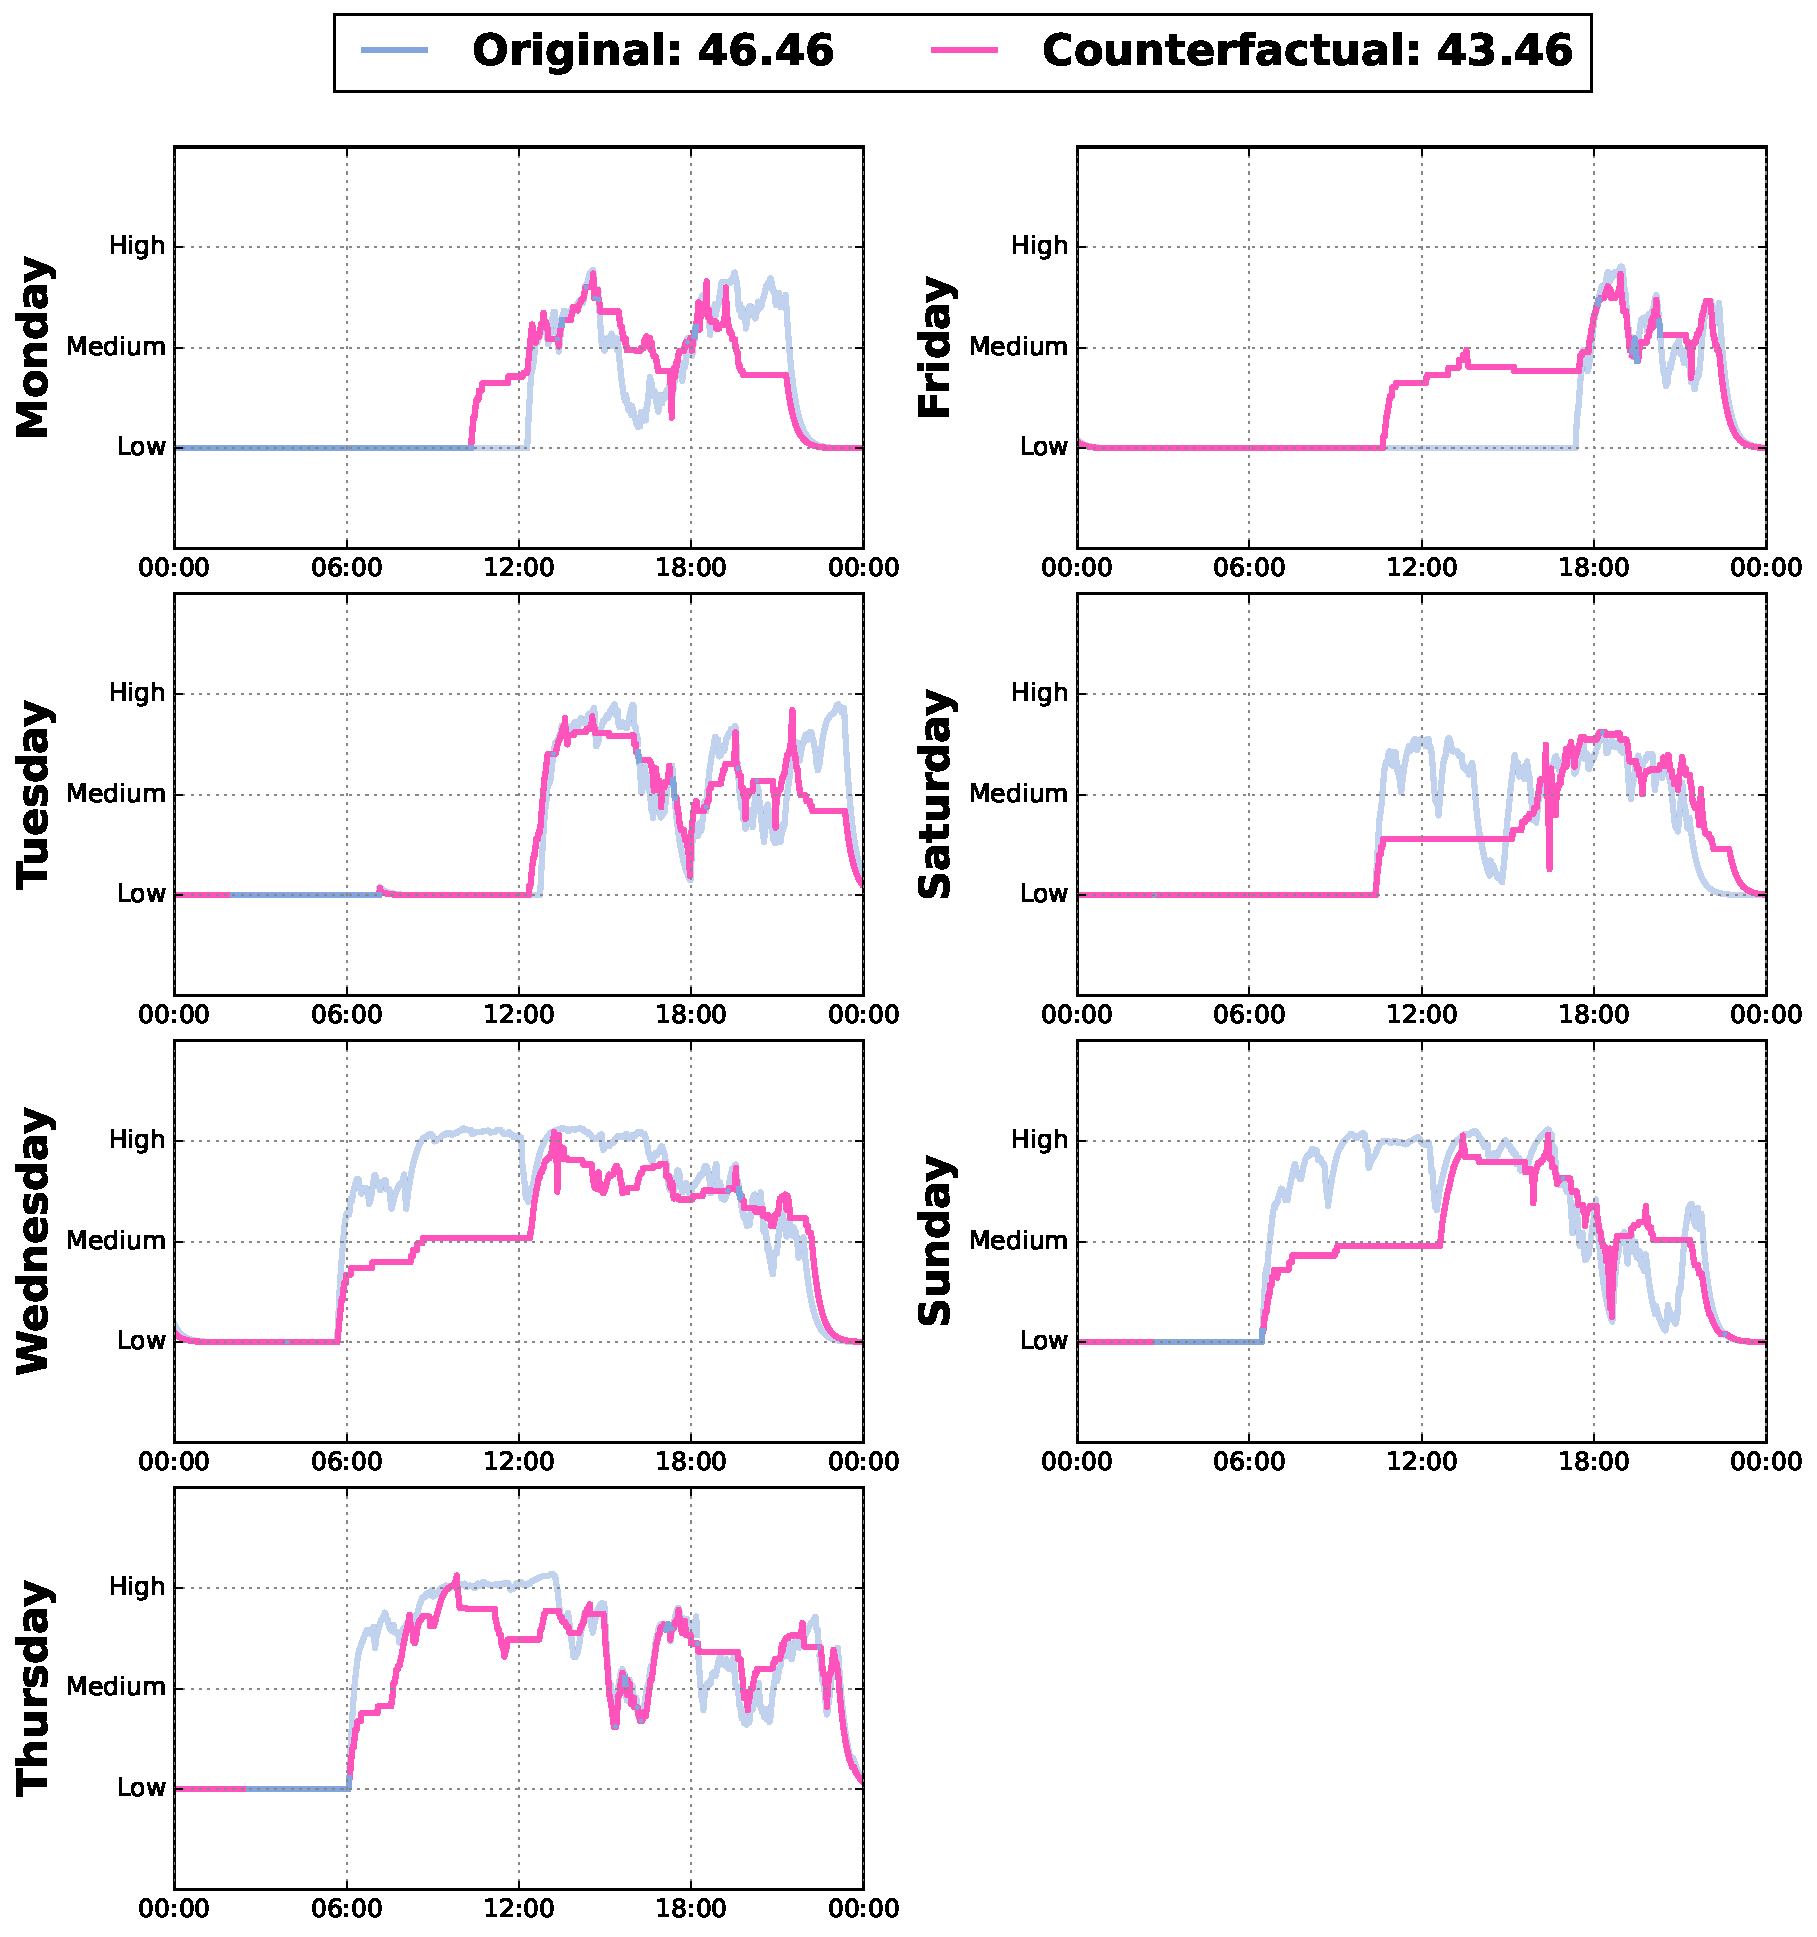
\includegraphics[width=\textwidth]{images/6306/1_6306_TCN_DBA_cf.pdf}
         \caption{DBAR Counterfactual}
         \label{fig:cf:dba}
     \end{subfigure}
    \hfill
     \begin{subfigure}[b]{0.24\textwidth}
         \centering
         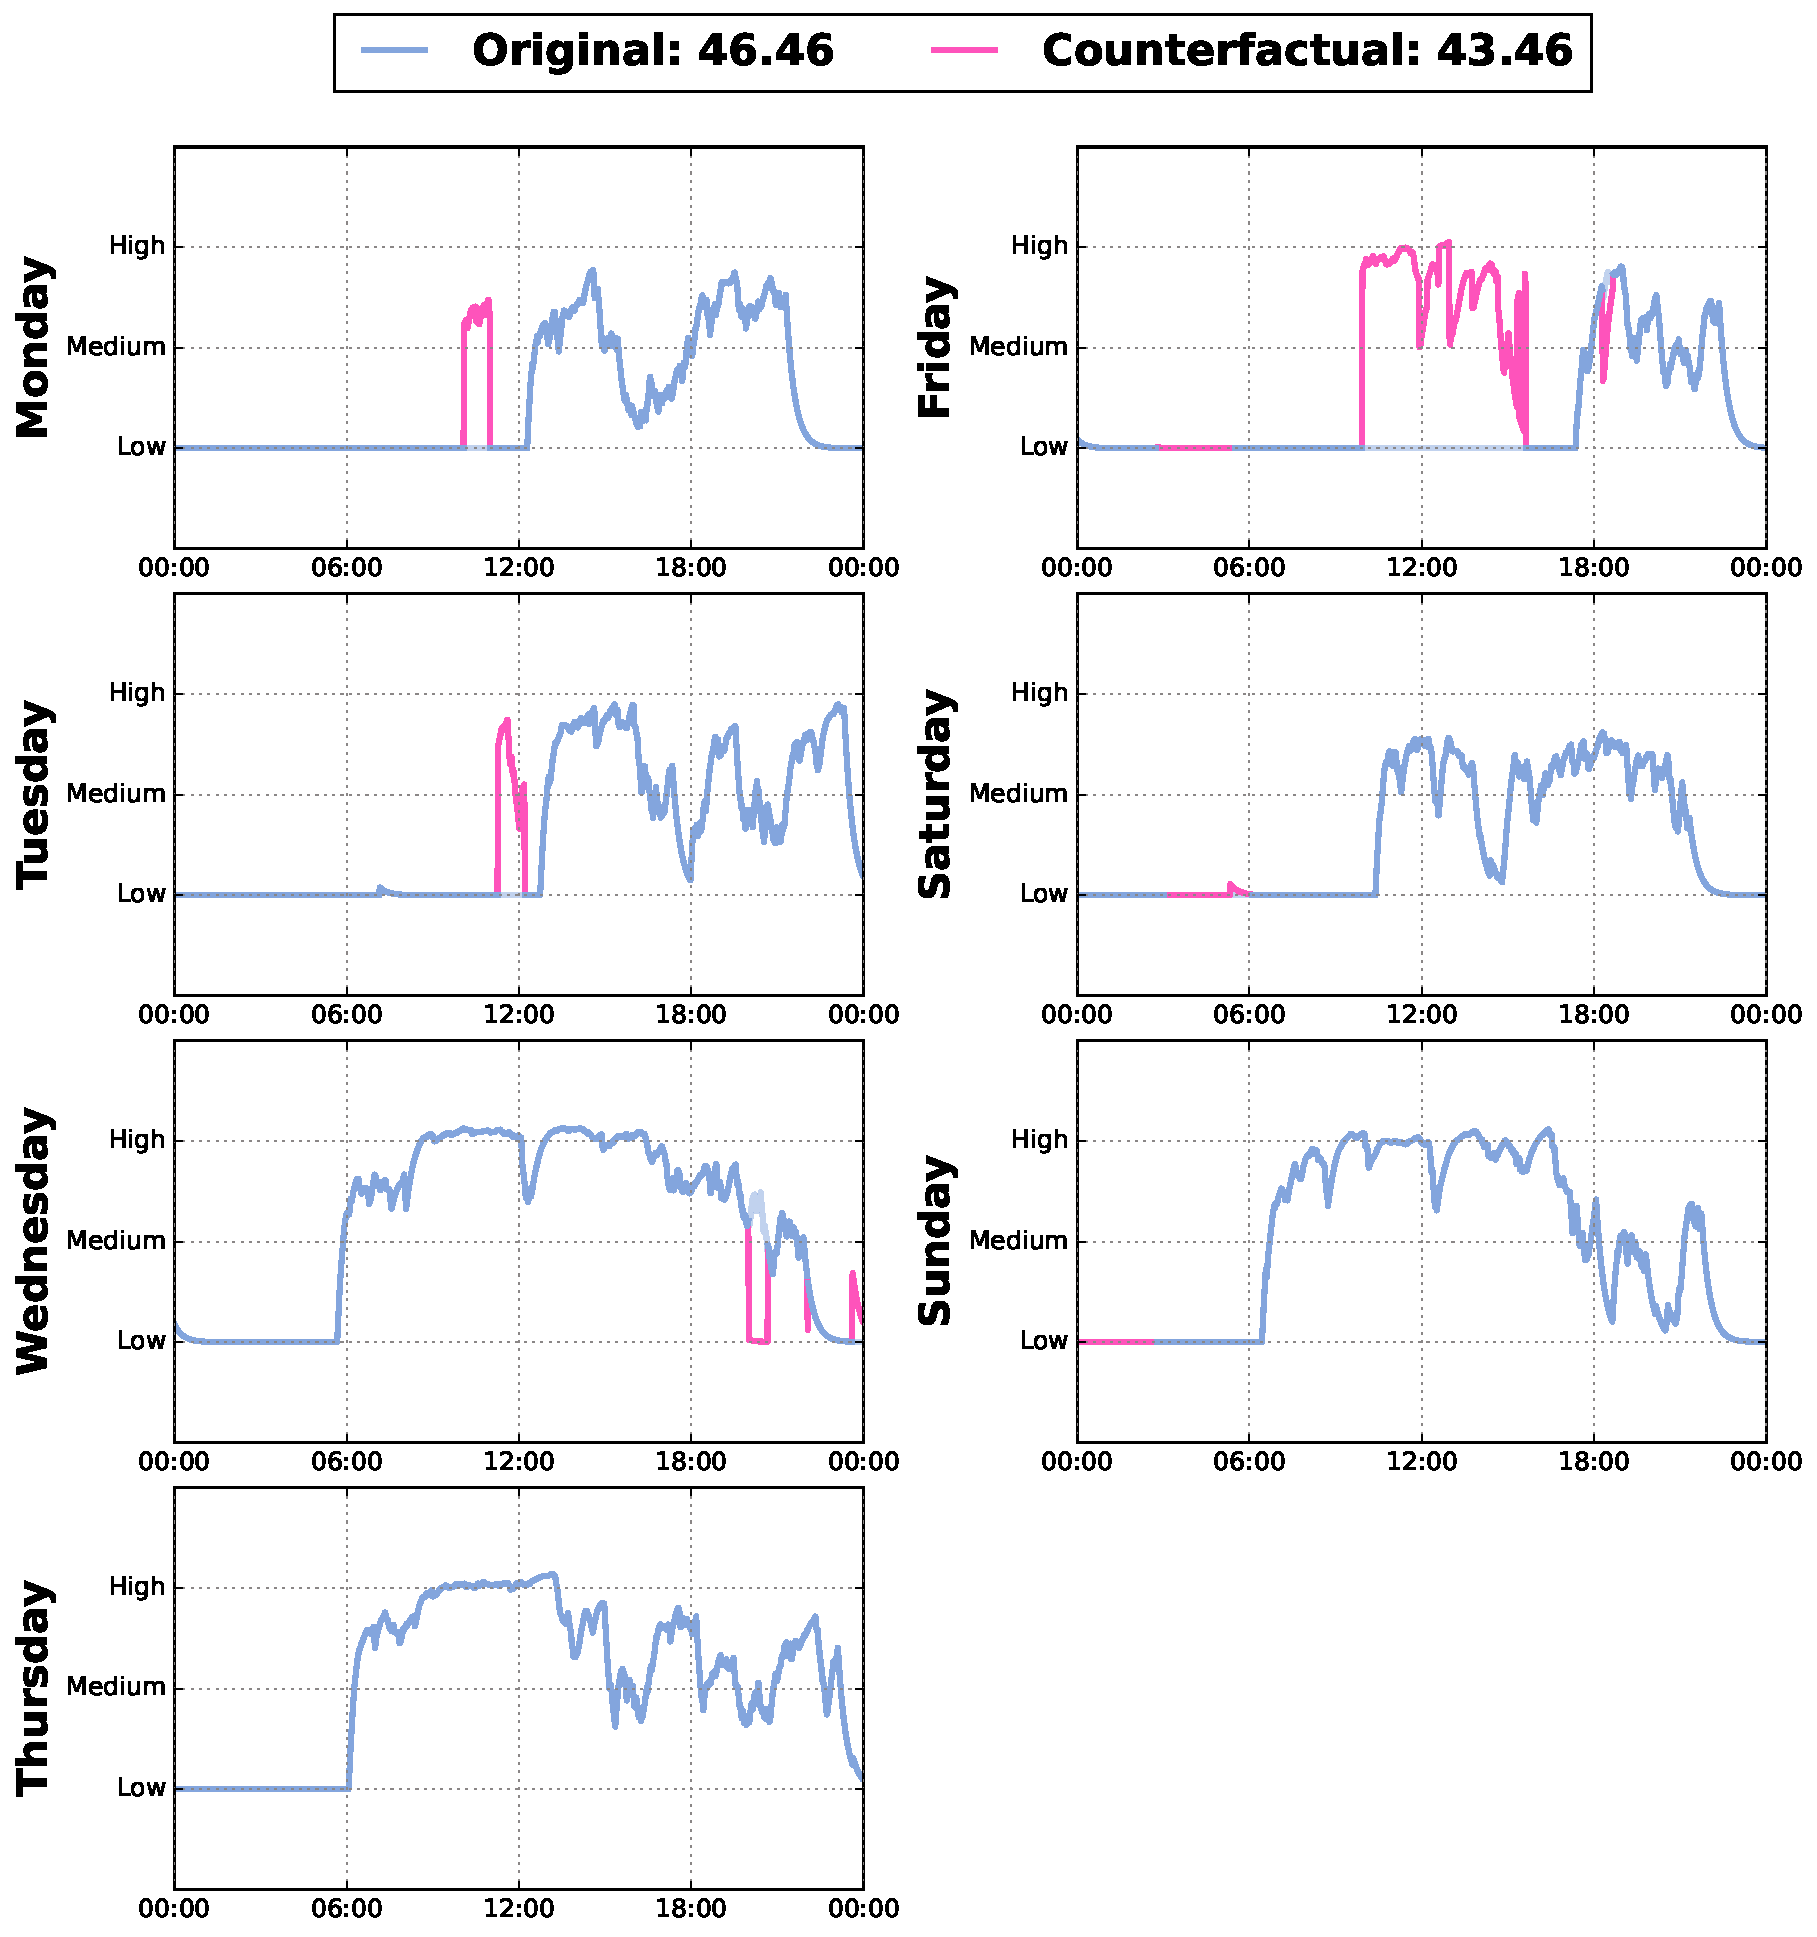
\includegraphics[width=\textwidth]{images/6306/2_6306_TCN_TSEvo_cf.pdf}
         \caption{TSEvoR Counterfactual}
         \label{fig:cf:tsevo}
     \end{subfigure}

          \begin{subfigure}[b]{0.24\textwidth}
         \centering
         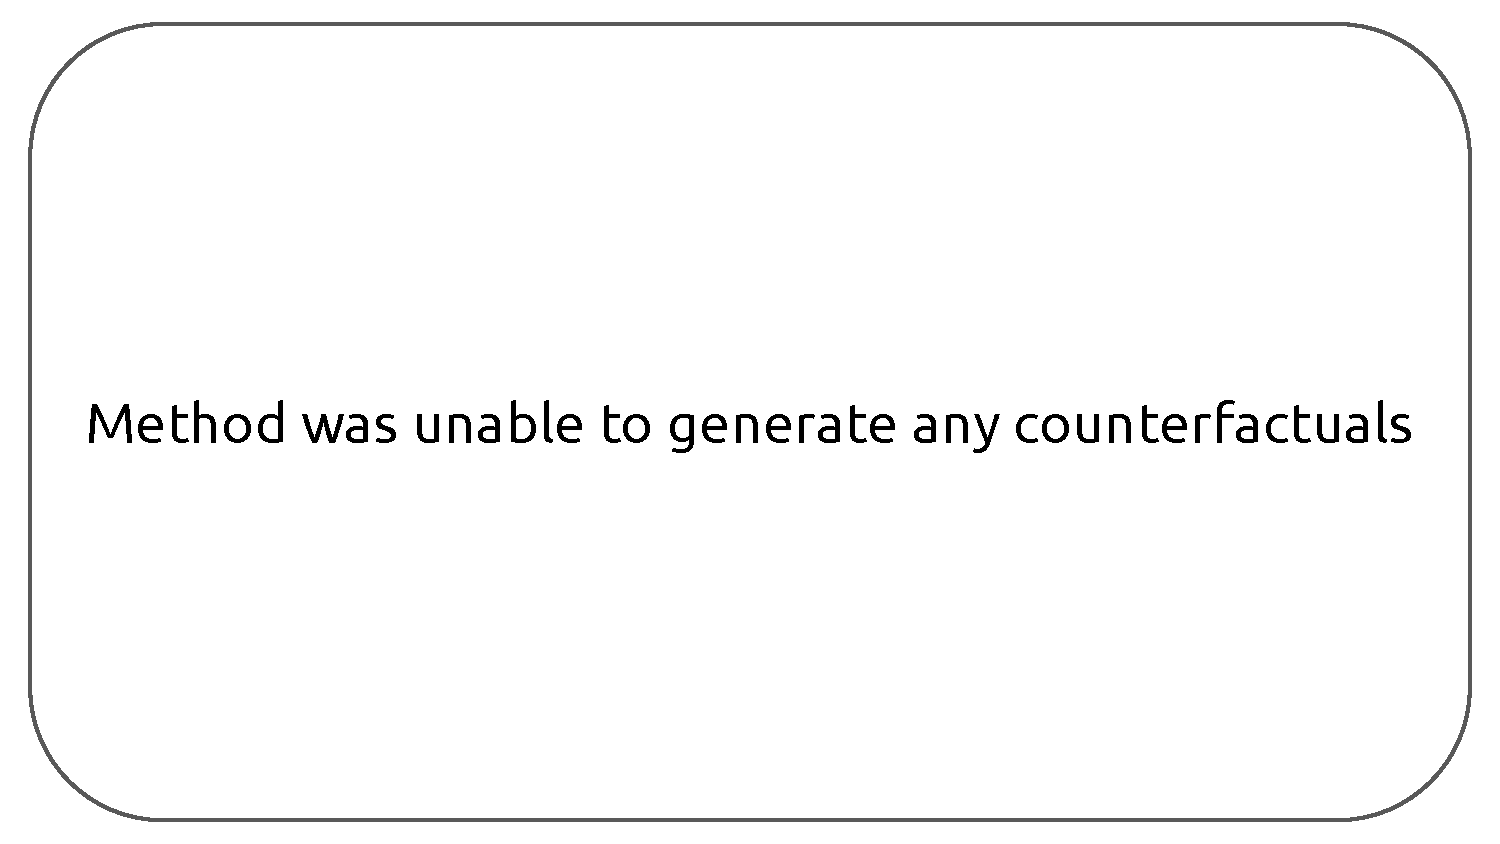
\includegraphics[width=\textwidth]{images/6306/0_6306_TCN_Wachter_reco.pdf}
         \caption{\gls{wachter} Recommendations}
         \label{fig:reco:wachter}
     \end{subfigure}
     \hfill
     \begin{subfigure}[b]{0.24\textwidth}
         \centering
         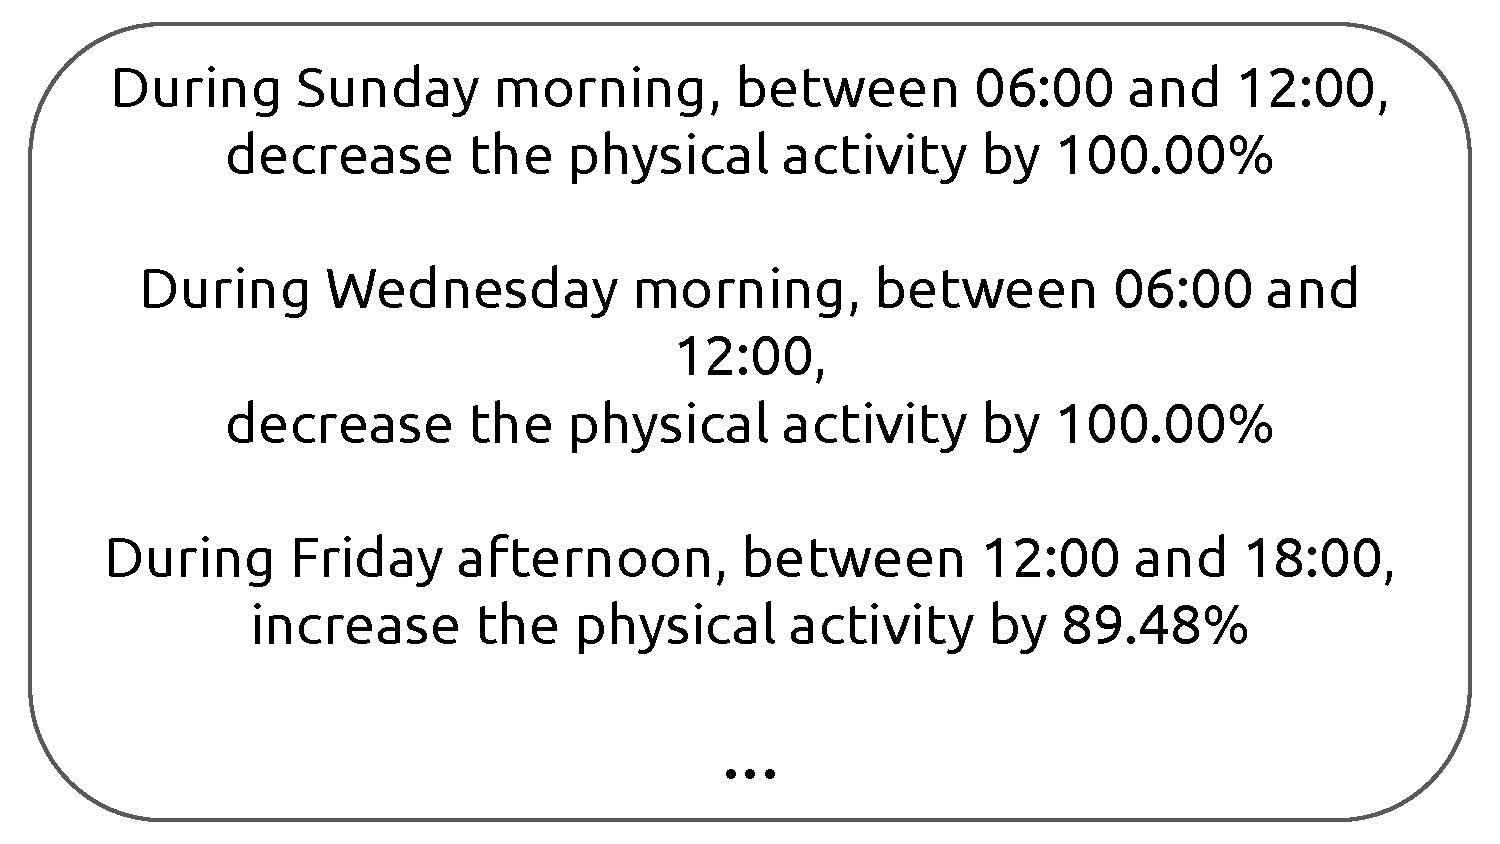
\includegraphics[width=\textwidth]{images/6306/4_6306_TCN_NUN_reco.pdf}
         \caption{NUNR Recommendations}
         \label{fig:reco:nun}
     \end{subfigure}
     \hfill
     \begin{subfigure}[b]{0.24\textwidth}
         \centering
         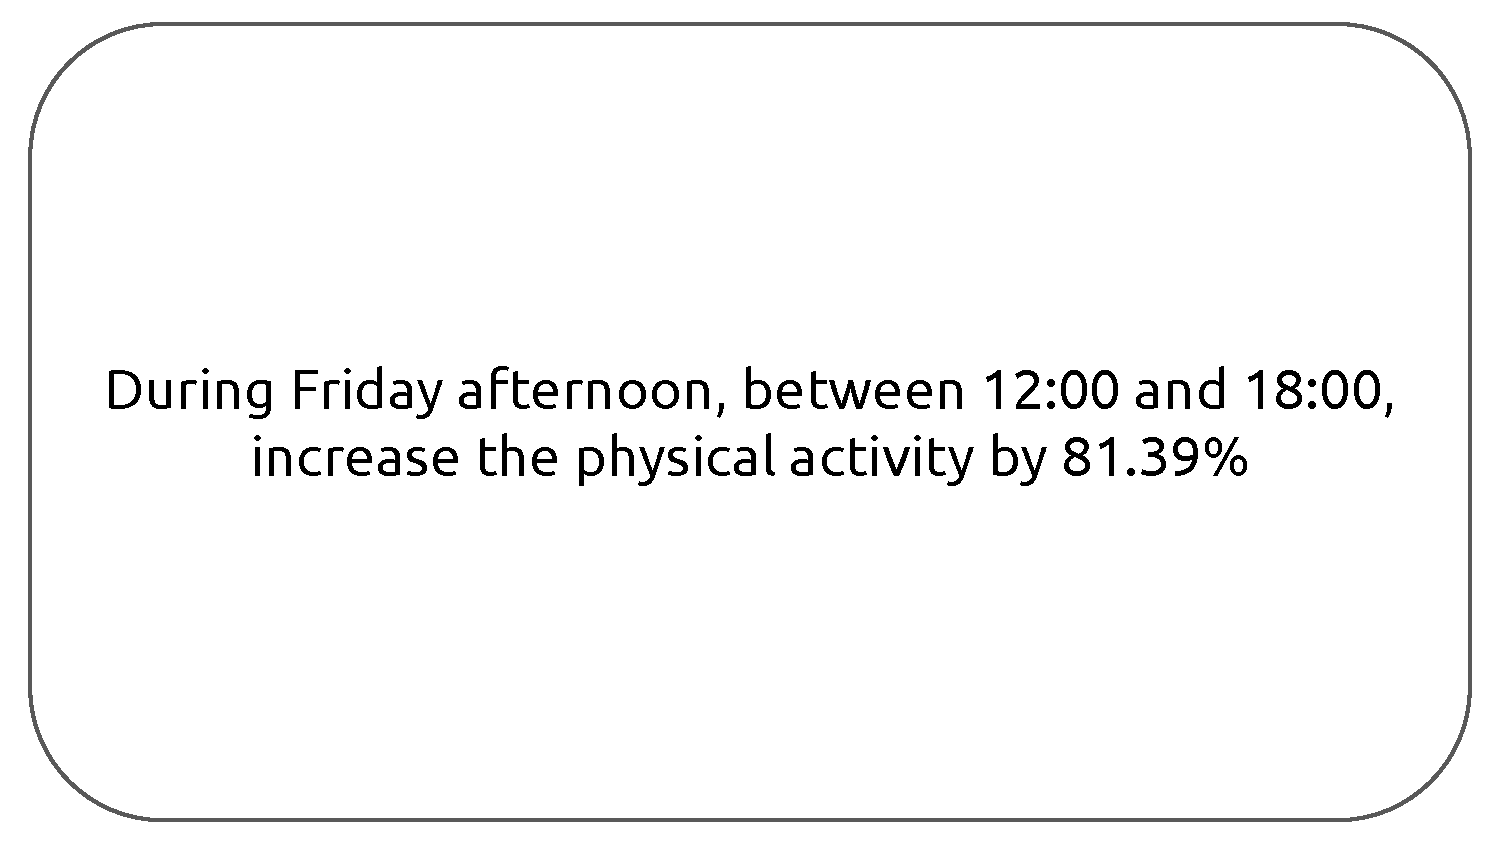
\includegraphics[width=\textwidth]{images/6306/1_6306_TCN_DBA_reco.pdf}
         \caption{DBAR Recommendations}
         \label{fig:reco:dba}
     \end{subfigure}
    \hfill
     \begin{subfigure}[b]{0.24\textwidth}
         \centering
         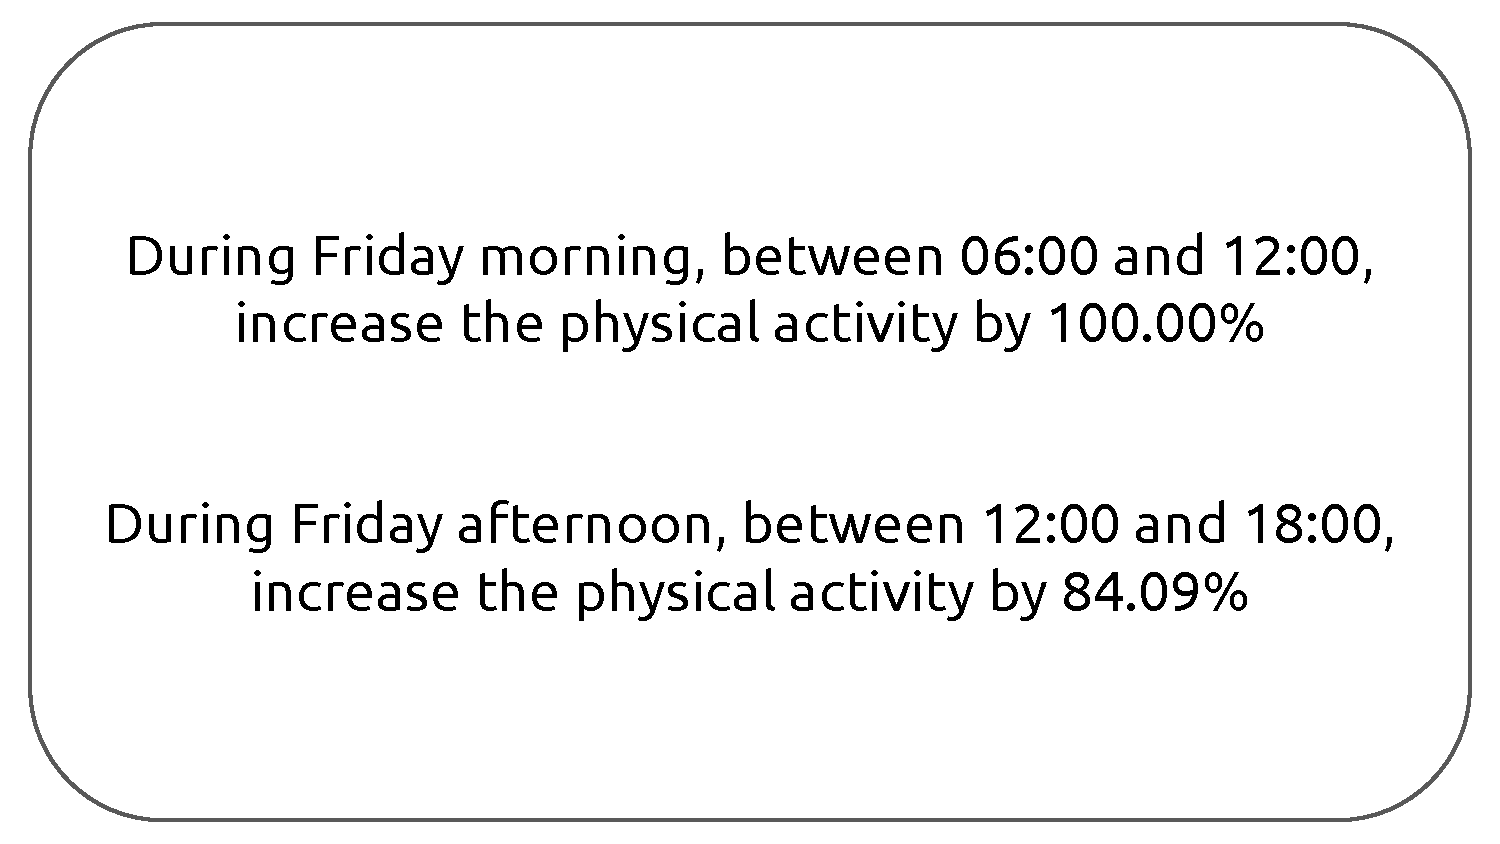
\includegraphics[width=\textwidth]{images/6306/2_6306_TCN_TSEvo_reco.pdf}
         \caption{TSEvoR Recommendations}
         \label{fig:reco:tsevo}
     \end{subfigure}

    \caption{Example of time series counterfactuals (pink line) of an input time
series (blue line) for the biological estimation problem, where, given a threshold $\varepsilon=3$, the counterfactual modifies the original activity so the DL model predicts a smaller biological age. Each plot represents a different counterfactual technique, and each corresponding text recommendation is listed below the plot.}
    \label{fig:quali-eval}
\end{figure*}

In the results section, we first report the performance of the \gls{dl} models to estimate Biological Age data~(cf.~Section~\ref{sec:results:dl-training}). Then, we evaluate the generated \gls{cfe} using qualitative and quantitative criteria~(cf.~Section~\ref{sec:results:cf}).

\subsection{Biological Age Estimation with Deep Learning}
\label{sec:results:dl-training}
We set out to reproduce results presented in prior work \cite{pyrkov_extracting_2018, rahman_deep_2019} that use \gls{dl} models to estimate biological age from physical activity data and achieved the following results~(cf.~Table~\ref{tab:models}).
In Rahman et al. work \cite{rahman_deep_2019}, the authors reported slightly different results. For the \gls{convlstm}, they reported a \gls{mae} of $13.21$ years, an \gls{mse} of $282,58$ with a Pearson correlation of $0.62$. For the \gls{cnn}, they reported an \gls{mae} of $15.49$, an \gls{mse} of $353.82$, and a Pearson correlation of $0.45$.
\begin{table}[h!]
    \centering
    \begin{tabular}{cccc}
        \toprule
        \textbf{Model} & \textbf{\gls{mse}$\,{}^\downarrow$} & \textbf{\gls{mae}$\,{}^\downarrow$} & \makecell{\textbf{Pearson} \\\textbf{Correlation}$\,{}^\uparrow$}\\
        \midrule
        \textbf{\gls{tcn}} & 367.69 & 14.85 & 0.49\\
        \textbf{\gls{cnn}} & 501.33 & 17.50 & 0.23\\
        \textbf{\gls{convlstm}} & 488.25 & 17.35 & 0.22\\
        \bottomrule
    \end{tabular}
    \caption{Comparison of the models' performances}
    \label{tab:models}
\end{table}

\subsection{Counterfactuals for Biological Age Estimation}
\label{sec:results:cf}
In this section, we evaluate the generated counterfactuals in two ways. First, qualitatively, we plotted one patient evaluated with the four different counterfactual techniques. The plots allow us to evaluate the user interpretability of the explanations. Looking at the explanations, a user should understand what he does well, what he could improve, and what impact it will have on his health. Then, we evaluate quantitatively using metrics based on the properties defined in Section \ref{sec:methods}. 

\subsubsection{Qualitative evaluation}
 Fig. \ref{fig:quali-eval} shows counterfactuals obtained for a specific patient using the four counterfactual methods. We highlight findings for each method in the following subsections.

\subsubsection{\gls{wachter}}
Figure~\ref{fig:cf:wachter} shows the counterfactual result for patient 6306. It was obtained using the \gls{tcn} model and the \gls{wachter} technique. The model's predicted biological labels are at the plot's top. According to the \gls{tcn} model, the patient's biological age is 46.46.
% \textbf{Contrastiveness} From the plot and the recommendations, it is not possible for the user to understand what changes are necessary to improve his biological age.\\
% \textbf{Selectivity} Again, the user cannot understand the explanations and the recommendations, which should be his main priority.\\
% \textbf{Social} \gls{wachter}'s changes are invisible on the plot. The user needs precise physical activity control to apply these changes; thus, the explanations are unrealistic. \\
% \textbf{Truthful} The counterfactual's level of physical activity is the same as the user's, which makes it plausible. \\
% \textbf{Consistent with prior beliefs} From the plot, the explanation suggests that having almost the same physical activity results in a drop of twelve years for the predicted biological age (!), which is not consistent with prior beliefs.\\
The counterfactual physical activity level corresponds to that of someone who is 34.1 years old, which is not a valid counterfactual, as valid counterfactuals need to have a biological age between 40.46 and 43.46 years old. The \gls{wachter} technique modifies slightly the physical activity recorded at every timestamp to find a counterfactual, resulting in hardly interpretable explanations. The explanations could not give any recommendations.

\subsubsection{\gls{nunr}}
Figure~\ref{fig:cf:nun} displays the counterfactual outcome for patient $6306$ using the \gls{tcn} model explained with the \gls{nunr} technique.
% \textbf{Contrastiveness} The \gls{nunr} technique requires a change in the patient's everyday routine. With the recommendations, the focus is on Sunday and Wednesday mornings and Friday afternoons. \\
% \textbf{Selectivity} The whole physical activity is highlighted, not only a subset. The text recommendations improve selectivity by giving the top three timestamps that should be changed.\\
% \textbf{Social} Based on the plot and the recommendations, the user has to change his habits most of the day of the week.\\
% \textbf{Truthful} Concretely, the \gls{nunr}-CF shows the physical activity of someone at least three years younger. So, as someone is doing this activity, the activity is plausible.\\
% \textbf{Consistent with prior beliefs} Recommendations mostly suggest that the user should decrease his physical activity, but it is a common belief that doing more physical activity is healthier overall.\\
The \gls{nunr} biological age is 42.39, which is a valid result. Based on the explanation, four recommendations were made to improve the patient's health; only the top three are shown in the plot. These include reducing activity levels on Wednesday and Sunday mornings and Saturday afternoons and increasing activity on Friday afternoons.

\subsubsection{\gls{dbar}}
Figure~\ref{fig:cf:dba} shows the counterfactual for patient $6306$ obtained through the \gls{tcn} model with the \gls{dbar} technique.
% \textbf{Contrastiveness} The plot only does not indicate necessary changes. When adding the recommendations, the focus on Friday becomes apparent.\\
% \textbf{Selectivity} Similar to \gls{nunr}, many data points are affected by the explanations, and again, the recommendation highlights the most important subset of the physical activity.\\
% \textbf{Social} Based on the plot and the recommendations, the user has to change his habits most of the day of the week. \\
% \textbf{Truthful} The DBA average introduces spikes in the physical activity.\\
% \textbf{Consistent with prior beliefs} The DBA averaging removed the main inconsistency in NUN recommendations, as the counterfactual no longer suggests decreasing physical activity. \\
The \gls{dbar} biological age is 43.46, which is an optimal and valid result. It is optimal because 43.46 is the closest accepted label possible. By comparing with the \gls{nunr} plot, we can observe that the \gls{dbar} technique averages between the \gls{nunr}'s physical activity and the patient's physical activity to produce a similar counterfactual, with less important changes (percentage changes are lower) but still slight changes at each time stamp. Based on the \gls{dbar}'s output, the recommender suggests only one recommendation to improve the patient's biological age: increasing physical activity on Friday afternoon. It is important to note that this was already a recommendation from the \gls{nunr} technique.

\subsubsection{\gls{tsevor}}
Figure~\ref{fig:cf:tsevo} shows a counterfactual for patient $6306$, which was obtained using the \gls{tcn} model and explained using the \gls{tsevor} technique.
% \textbf{Contrastiveness} The plot highlights a large area on Friday and three smaller areas on Monday, Tuesday, and Wednesday. This is then narrowed to only Friday by the text recommendation.\\
% \textbf{Selectivity} From the plot, the user observes three main changes: Monday morning, Tuesday morning, and Friday midday. The recommendation helps the user select Friday as the main area of focus.\\
% \textbf{Social} The recommendations are realistic as they focus mainly on one day. \\
% \textbf{Truthful} The counterfactual's physical activity is plausible. \\
% \textbf{Consistent with prior beliefs} The explanations suggest increasing physical activity on a day when the user had very little activity. \\
The \gls{tsevor} biological age is 43.46, which is an optimal and valid result. \gls{tsevor} only had to make a few changes to the timestamps to arrive at a valid and optimal result. Based on this analysis, it then recommended that the patient increase their physical activity on Friday morning and afternoon, which is the same as \gls{dbar} and \gls{nunr}.


\subsection{Quantitative evaluation}
\begin{table*}[h!]
    \large
    \caption{Objectives}
    \centering
    \resizebox{0.96\textwidth}{!}{
        \small
        \begin{tabular}{@{ }l@{\hspace{4mm}}l@{\hspace{7mm}}c@{\hspace{10mm}}l@{\hspace{10mm}}l@{\hspace{10mm}}l@{\hspace{10mm}}c@{\hspace{10mm}}}
                \toprule[1pt]%    
                && \textbf{Validity}$\,{}^\uparrow$& \textbf{Proximity}$\,{}^\downarrow$& \textbf{Sparsity}$\,{}^\downarrow$& \textbf{Plausibility}$\,{}^\uparrow$& \textbf{Time}$\,{}^\downarrow$
                    \\
                    \midrule%
                \multirow{4}{*}{\textbf{\rotatebox{90}{CNN$\,\;$}}}\n& \textbf{TSEvoR}& 0.37±0.48& 159.99±274.71& \textbf{0.04±0.09}& 0.39±0.25& 8m01s±02m52s\\& \textbf{NUNR}& \textbf{0.99±0.08}& 4740.66±1149.04& 0.98±0.02& \textbf{0.47±0.20}& \textbf{0m01s±00m01s}\\& \textbf{DBAR}& 0.10±0.31& 2499.74±702.91& 0.99±0.03& 0.02±0.11& 9m28s±04m58s\\& \textbf{\gls{wachter}}& 0.00±0.00& \textbf{0.00±0.00}& 1.00±0.00& 0.00±0.00& 1m01s±00m28s\\\n\bottomrule[1pt]\multirow{4}{*}{\textbf{\rotatebox{90}{ConvLSTM$\,\;$}}}\n& \textbf{TSEvoR}& 0.08±0.27& 450.75±445.8& \textbf{0.07±0.10}& 0.46±0.29& 47m36s±11m21s\\& \textbf{NUNR}&\textbf{0.99±0.08}& 3944.03±796.31& 0.98±0.02& \textbf{0.59±0.25}& \textbf{00m01s±00m01s}\\& \textbf{DBAR}& 0.09±0.29& 1898.02±328.64& 1.00±0.02& 0.04±0.15& 11m33s±04m32s\\& \textbf{\gls{wachter}}& 0.02±0.12& \textbf{0.00±0.00}& 0.99±0.02& 0.14±0.27& 06m32s±01m48s\\\n\bottomrule[1pt]\multirow{4}{*}{\textbf{\rotatebox{90}{TCN$\,\;$}}}\n& \textbf{TSEvoR}& 0.39±0.49& 147.37±242.41& \textbf{0.04±0.09}& 0.41±0.26& 10m01s±01m14s\\& \textbf{NUNR}& \textbf{0.99±0.08}& 4740.66±1149.04& 0.98±0.02& \textbf{0.51±0.23}& \textbf{00m01s±00m01s}\\& \textbf{DBAR}& 0.10±0.30& 2344.37±639.02& 1.00±0.02& 0.01±0.07& 12m03s±05m54s\\& \textbf{\gls{wachter}}& 0.00±0.00& \textbf{0.00±0.00}& 1.00±0.00& 0.00±0.00& 01m09s±00m03s\\
            \bottomrule[1pt]
            \end{tabular}
    }
    \label{tab:experiments:results}
    \vspace{-5mm}
\end{table*}



% \begin{table*}[!t]

%                 \caption{Objectives}

%                 \centering

%                 \resizebox{0.96\textwidth}{!}{%


%                 \begin{tabular}{@{ }l@{\hspace{2mm}}l@{\hspace{7mm}}c@{\hspace{1.5mm}}c@{\hspace{1mm}}c@{\hspace{7mm}}c@{\hspace{1.5mm}}c@{\hspace{1mm}}c@{\hspace{7mm}}c@{\hspace{1.5mm}}c@{\hspace{1mm}}c@{\hspace{7mm}}c@{\hspace{1.5mm}}c@{\hspace{1mm}}c@{\hspace{7mm}}c@{\hspace{1.5mm}}c@{\hspace{1mm}}c@{}}

%                 \toprule[1pt]%

%                 && \multicolumn{3}{c@{\hspace{10mm}}}{\textbf{Validity}$\,{}^\uparrow$}& \multicolumn{3}{c@{\hspace{10mm}}}{\textbf{Proximity}$\,{}^\downarrow$}& \multicolumn{3}{c@{\hspace{10mm}}}{\textbf{Sparsity}$\,{}^\downarrow$}& \multicolumn{3}{c@{\hspace{10mm}}}{\textbf{Plausibility}$\,{}^\uparrow$}& \multicolumn{3}{c@{\hspace{10mm}}}{\textbf{Time}$\,{}^\downarrow$}\\ 
% [1mm]
% && \textbf{CNN}& \textbf{ConvLSTM}& \textbf{TCN}& \textbf{CNN}& \textbf{ConvLSTM}& \textbf{TCN}& \textbf{CNN}& \textbf{ConvLSTM}& \textbf{TCN}& \textbf{CNN}& \textbf{ConvLSTM}& \textbf{TCN}& \textbf{CNN}& \textbf{ConvLSTM}& \textbf{TCN}\\ 
% \midrule%
% \multirow{4}{*}{\textbf{\rotatebox{90}{Techniques$\,\;$}}}
% & TSEvoR 	& 0.37 	& 0.08 	& 0.39 	& 159.99 	& 450.75 	& \textbf{147.37} 	& \textbf{0.04} 	& 0.07 	& \textbf{0.04} 	& 0.39 	& 0.46 	& 0.41 	& 08m 01s 	& 47m 36s 	& 10m 01s \\
% & NUNR 	& \textbf{0.99} 	& \textbf{0.99} 	& \textbf{0.99} 	& 4740.66 	& 3944.03 	& 4740.66 	& 0.98 	& 0.98 	& 0.98 	& 0.47 	& \textbf{0.59} 	& 0.51 	& \textbf{00m 00s} 	& \textbf{00m 00s} 	& \textbf{00m 00s} \\
% & DBAR 	& 0.1 	& 0.09 	& 0.1 	& 2499.74 	& 1898.02 	& 2344.37 	& 0.99 	& 1.0 	& 1.0 	& 0.02 	& 0.04 	& 0.01 	& 12m 28s 	& 11m 33s 	& 12m 03s \\
% & \gls{wachter} 	& 0.0 	& 0.0 	& 0.0 	& - 	& - 	& - 	& 1.0 	& 1.0 	& 1.0 	& 0.0 	& 0.0 	& 0.0 	& 01m 01s 	& 07m 13s 	& 01m 19s \\

%                 \bottomrule[1pt]

%                 \end{tabular}

%                 }

%                 \label{tab:experiments:results}

%                 \vspace{-5mm}

%                 \end{table*}


% \begin{table*}[!t]

%     \caption{Objectives}

%                 \centering

%                 \resizebox{0.96\textwidth}{!}{%


%                 \begin{tabular}{@{ }l@{\hspace{2mm}}l@{\hspace{7mm}}c@{\hspace{1.5mm}}c@{\hspace{1mm}}c@{\hspace{7mm}}c@{\hspace{1.5mm}}c@{\hspace{1mm}}c@{\hspace{7mm}}c@{\hspace{1.5mm}}c@{\hspace{1mm}}c@{\hspace{7mm}}c@{\hspace{1.5mm}}c@{\hspace{1mm}}c@{\hspace{7mm}}c@{\hspace{1.5mm}}c@{\hspace{1mm}}c@{}}

%                 \toprule[1pt]%

%                 && \multicolumn{3}{c@{\hspace{10mm}}}{\textbf{Validity}$\,{}^\uparrow$}& \multicolumn{3}{c@{\hspace{10mm}}}{\textbf{Proximity}$\,{}^\downarrow$}& \multicolumn{3}{c@{\hspace{10mm}}}{\textbf{Sparsity}$\,{}^\downarrow$}& \multicolumn{3}{c@{\hspace{10mm}}}{\textbf{Plausibility}$\,{}^\uparrow$}& \multicolumn{3}{c@{\hspace{10mm}}}{\textbf{Time}$\,{}^\downarrow$}\\ 
% [1mm]
% && \textbf{CNN}& \textbf{ConvLSTM}& \textbf{TCN}& \textbf{CNN}& \textbf{ConvLSTM}& \textbf{TCN}& \textbf{CNN}& \textbf{ConvLSTM}& \textbf{TCN}& \textbf{CNN}& \textbf{ConvLSTM}& \textbf{TCN}& \textbf{CNN}& \textbf{ConvLSTM}& \textbf{TCN}\\ 
% \midrule%
% \multirow{4}{*}{\textbf{\rotatebox{90}{Techniques$\,\;$}}}
% & TSEvoR 	& 0.37±0.48 	& 0.08±0.27 	& 0.39±0.49 	& 159.99±274.71 	& 450.75±445.8 	& 147.37±242.41 	& 0.04±0.09 	& 0.07±0.1 	& 0.04±0.09 	& 0.39±0.25 	& 0.46±0.29 	& 0.41±0.26 	& 08m 01s±02m 52s 	& 47m 36s±11m 21s 	& 10m 01s±01m 14s \\
% & NUNR 	& 0.99±0.08 	& 0.99±0.08 	& 0.99±0.08 	& 4740.66±1149.04 	& 3944.03±796.31 	& 4740.66±1149.04 	& 0.98±0.02 	& 0.98±0.02 	& 0.98±0.02 	& 0.47±0.2 	& 0.59±0.25 	& 0.51±0.23 	& 00m 00s±00m 00s 	& 00m 00s±00m 00s 	& 00m 00s±00m 00s \\
% & DBAR 	& 0.1±0.31 	& 0.09±0.29 	& 0.1±0.3 	& 2499.74±702.91 	& 1898.02±328.64 	& 2344.37±639.02 	& 0.99±0.03 	& 1.0±0.02 	& 1.0±0.02 	& 0.02±0.11 	& 0.04±0.15 	& 0.01±0.07 	& 12m 28s±04m 58s 	& 11m 33s±04m 32s 	& 12m 03s±04m 54s \\
% & \gls{wachter} 	& 0.0±0.0 	& 0.0±0.0 	& 0.0±0.0 	& -±- 	& -±- 	& -±- 	& 1.0±0.0 	& 1.0±0.0 	& 1.0±0.0 	& 0.0±0.0 	& 0.0±0.0 	& 0.0±0.0 	& 01m 01s±00m 27s 	& 07m 13s±00m 42s 	& 01m 19s±00m 03s \\

%                 \bottomrule[1pt]

%                 \end{tabular}

%                 }

%                 \label{tab:experiments:results}

%                 \vspace{-5mm}

% \end{table*}


We generated counterfactuals on the 723 samples from the test set. To generate counterfactuals, we first feed each sample from the test set to each of the three deep-learning models (\gls{cnn}, \gls{tcn}, and \gls{convlstm}). We then generated counterfactuals using the four different counterfactual techniques (\gls{wachter}, \gls{nunr}, \gls{dbar}, and \gls{tsevor}). Finally, we evaluate the $723\times3\times4=8676$ generated counterfactuals with the following metrics:
\begin{itemize}
    \item \textbf{Validity}: Proportion of the 723 generated counterfactuals that are valid~(cf.~Def.~\ref{def:validity}). 
    \item \textbf{Proximity}: $L_1$ norm (Manhattan distance) between the query $x$ and the counterfactual $x^{cf}$.
    \begin{equation}
        ||x - x^{cf}||_1 = \sum_i|x_i - x_i^{cf}|
    \end{equation}
    \item \textbf{Sparsity}: Proportion of changed data points to obtain the counterfactual. 
    \item \textbf{Plausibility}: Proportion of Nearest Neighbours with a label close to the counterfactual label. We used $k=5$ \gls{nn}, and $\varepsilon=3$ as the threshold value to differentiate between close and far neighbors.
    \begin{equation}        \text{Plausibility}=\frac{1}{k}\sum_{i\, \in\, kNN(x^{cf})}\mathbbm{1}_{|y_i - y^{cf}|\, \leq\, \varepsilon}
    \end{equation}
    \item \textbf{Time}: Time needed to explain a sample.
\end{itemize}

Upon analysis, we can first observe that the best-performing explainable technique for each metric remains constant across the models, which only impacts the time aspect. Secondly, we note that the \gls{nunr} technique performs best across three out of five metrics but falls short on the proximity and sparsity metrics. Compared to \gls{nunr}, \gls{dbar} improves the proximity metric at the cost of a large drop in validity and plausibility. Thirdly, it is evident that all techniques, except for \gls{tsevor}, cannot produce sparse counterfactuals. It is also important to note that \gls{tsevor} ranks first or second in every metric except for time, where it secures third place. Moreover, when using \gls{tsevor}, the model plays a role in the validity and time metrics. Indeed, the validity drops to 0.08 when explaining the \gls{convlstm} model, compared to 0.37 for \gls{cnn} and 0.39 for \gls{tcn}, while being five times slower.